\mysection{Guarding}{combat-guarding}

  \flavor{Go that way, really fast. If something gets in your way, turn. \\~ \Tilde Charles de Mar, \myital{Better Off Dead}}


  It is generally considered a \myital{really good idea} to avoid getting struck by claws, swords, and falling debris. Guarding is when you roll your dice to see if you are able to avoid getting hit by the Monster you're in combat with.

  \formula{Guarding Try}{
    \RO : Your \DEX \PLUS Monster Weakness \PLUS Your \LVL
  }



  To see if you can dodge the Monster, you must \RO with a Guarding try.  To make a Guarding try, roll your \DEX with the Monster's \mylink{Weakness}{monster-weakness}, and add your \LVL to the result. If you fall short, you can try to bump your die roll above a 19 by rolling various other dice (the Sellsword's \mylink{Prowess}{sellsword-prowess}, the associated die of your \mylink{Personality}{adventurer-personality}, etc.)

  If you fail in your Guarding try, you take damage from the Monster.

  \myhighlight{Taking Damage}{combat-taking-damage}

  Taking damage works in roughly the same way as dealing damage, except the Arbiter rolls for Monster damage.  \mybold{Monsters cannot Crit or Fumble}. The Arbiter is encouraged to roll the damage out in the open. The \SUM of the damage is applied to your Adventurer Sheet in the order specified to the right.

\cbreak

\begin{center}
  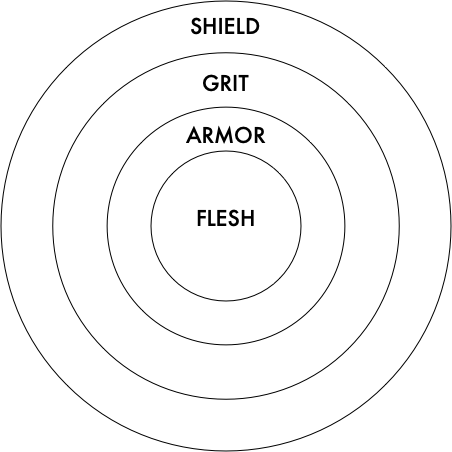
\includegraphics{combat/THE_ORDER}
\end{center}

  \mynumlist {
    \item \mybold{Shield} : If you have a shield equipped (that is, on your arm) and take \mybold{physical damage}, and you haven't taken a Combat Action yet, you can \mylink{Sunder}{combat-deeds-sunder} your shield. Stop here.  Otherwise ...
    \item \mybold{Grit} : Subtract the damage from your Grit.  If there's any damage left over, move to Armor i.e. if I have a Grit of 4 and I take 9 damage, I have 5 damage left over and I move on to Armor.
    \item \mybold{Armor} : If you have armor, see how much damage it will absorb.  Roll the \UD for your armor and subtract the result from the damage.  For example, if I'm wearing chain mail (Medium armor) I roll a d8; if I rolled a 5, I'd subtract 5 from the total damage. If I roll a Failure with my Armor, I still subtract the damage, but move the \UD \DCDOWN. If there's any damage left over, move onto Flesh.
    \item \mybold{Flesh} : Subtract the rest of the damage from Flesh. If you go to 0 or less Flesh, you are \mylink{Dying}{combat-dying}.
  }
